\subsection{Wonder 3D}\label{Wonder3D}

\citeauthor{long2023wonder3d} introduce Wonder3D, a technique that stands apart  from its predecessors primarily through its adeptness in generating not just color images, but also consistent multi-view normal maps. This method leverages a cross-domain diffusion model, ``extends the stable diffusion framework to model the joint distribution of two different domains, i.e., normals and colors'' \citep{long2023wonder3d}.


\begin{figure}[ht]
  \centering
    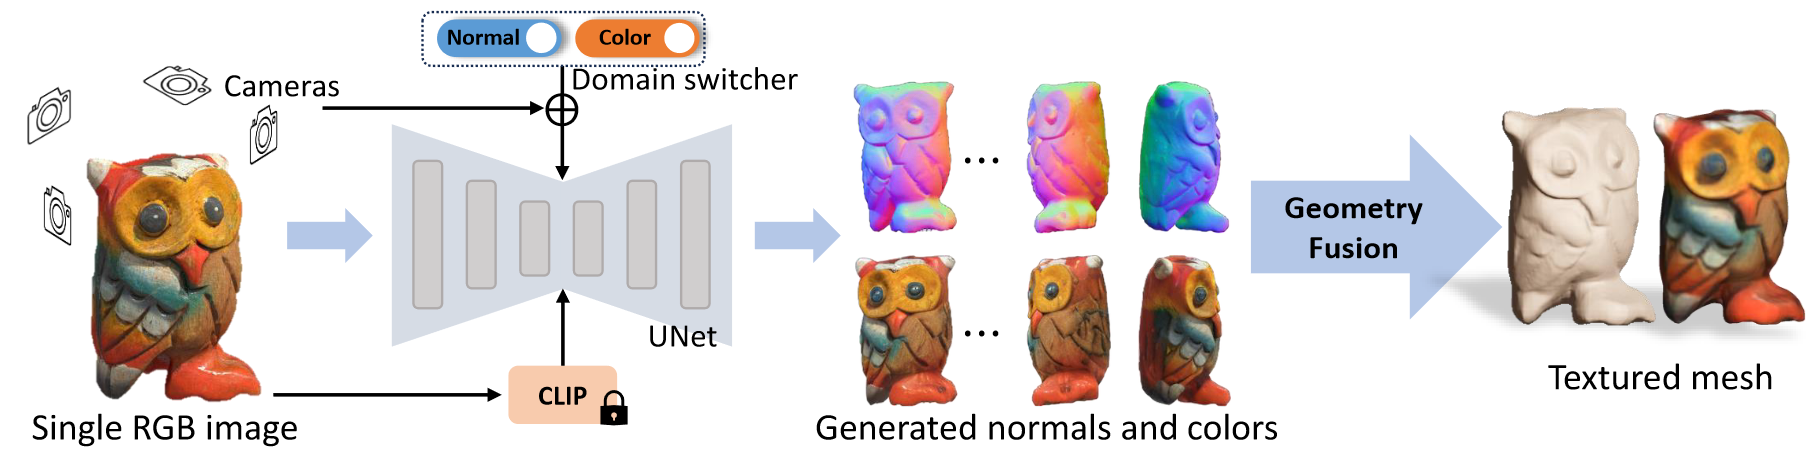
\includegraphics[width=1\columnwidth]{figures/Wonder3D.png}
    \caption{Summarized functionality of Wonder3D, depicting the method's unique approach to generating high-fidelity textured meshes from single images using cross-domain diffusion models \citep{long2023wonder3d}.}\label{fig:Wonder3D}
\end{figure}

The process of generating 3D models from images starts by using CLIP \citep{radfordCLIP} to get a textual description of the image.  

In Wonder3D, the formulation of 3D models is distinctively characterized by modeling the distribution of 3D assets \(p_a{(z)}\) ``as a joint distribution of its corresponding 2D multi-view normal maps and corresponding color images'' \citep{long2023wonder3d}. This modeling allows their training on 2D diffusion models \citep{long2023wonder3d}. The model, conditioned on a given image \( y \), aims to produce multiple normal maps \( n^{1:K} \) and color images \( x^{1:K} \) from various camera perspectives \((\pi_1, \pi_2, \ldots, \pi_k)\), which is achieved by employing a model \( f \), mathematically defined by \citeauthor{long2023wonder3d} as \((n^{1:K}, x^{1:K} | y) = f(y, \pi_{1:k})\).

The creation of the cross-domain joint distribution in Wonder3D is facilitated using a Markov chain within a diffusion framework.~\citeauthor{long2023wonder3d} formally represent this as \[ p\left(n_T^{(1: K)}, x_T^{(1: K)}\right) \prod_t p_\theta\left(n_{t-1}^{(1: K)}, x_{t-1}^{(1: K)} \mid n_t^{(1: K)}, x_t^{(1: K)}\right) \] where \( p\left(n_T^{(1: K)}, x_T^{(1: K)}\right) \) comprises Gaussian noises \citep{long2023wonder3d}.

The model also further enhances its functionality with the generation of consistent multi-view images. This addresses a notable challenge faced by earlier 2D diffusion models, which often produced images with geometric and visual inconsistencies across different views \citep{long2023wonder3d}.

Simply adapting pre-trained stable diffusion models to also output both normal maps and color images, encountered issues with slow convergence and poor generalization \citep{long2023wonder3d}. To address these challenges, Wonder3D introduce a cross-domain diffusion scheme named Domain Switcher \(s\), which is given as an extra input to the diffusion model \citep{long2023wonder3d}. \[
  n^{1:K}, x^{1:K} = f(y, \pi_{1:K}, s_n), f(y, \pi_{1:K}, s_c)
\] This equation by \citeauthor{long2023wonder3d} means that the model uses the switcher \( s \) to determine whether to generate normal maps (\( s_n \)) or color images (\( s_c \)), based on the input provided. However, only using the domain swither does not inherently guarantee geometric consistency between the color image and the normal map for a single view \citep{long2023wonder3d}. To ensure this consistency, Wonder3D employs cross-domain attention, allowing for information exchange between multiple domains, ensuring that the generated normal maps and color images for a particular view are geometrically aligned \citep{long2023wonder3d}.

To transform the 2D normal maps and color images into explicit 3D geometry, Wonder3D optimizes a neural implicit signed distance field (SDF) using a novel optimization scheme. Previous attempts proved challenging due to the sparse nature of the generated views and the subtle inaccuracies in the generated normal maps and color images, leading to distorted geometries, outliers, and incompleteness in the 3D models \citep{long2023wonder3d}.



To overcome these issues, Wonder3D introduces a novel geometric-aware optimization scheme. The optimization process involves segmenting object masks \( M_{0:N} \) from the normal maps \( G_{0:N} \) or color images \( H_{0:N} \) and performing optimization by ``randomly sampling a batch of pixels and their corresponding rays in world space [\(\ldots\)]'' \citep{long2023wonder3d}.

\citeauthor{long2023wonder3d} define the overall objective function as: \[ L = L_{normal} + L_{rgb} + L_{mask} + R_{eik} + R_{sparse} + R_{smooth} \]

The normal loss term, \( L_{normal} \), is key for aligning the 3D geometry with the generated normal maps. It employs a cosine function to maximize the similarity between the normals of the signed distance field (SDF) and the generated normals. The \( L_{rgb} \) term is a mean squared error loss that evaluates the difference between the rendered colors and the generated colors from the model. This term ensures that the color representation in the 3D model closely matches the original images. The \( L_{mask} \) term, a binary cross-entropy loss, calculates the errors between the rendered and generated masks. The eikonal regularization term, \( R_{eik} \), encourages the magnitude of the SDF gradients to maintain unit length, which is important for the stability of the shape's representation. The sparsity regularization term, \( R_{sparse} \), helps avoid isolated, floating parts in the SDF, ensuring a coherent and unified 3D structure. Finally, the smoothness regularization term, \( R_{smooth} \), enforces the smoothness of the SDF gradients in 3D space, contributing to the seamless and natural appearance of the 3D geometry.
